% Copyright © 2017-2018 Martin Ueding <dev@martin-ueding.de>
% Licensed under CC-BY 4.0

\documentclass{scrartcl}

\pagestyle{empty}

\usepackage{tikz}
\usetikzlibrary{arrows.meta, calc}

\begin{document}

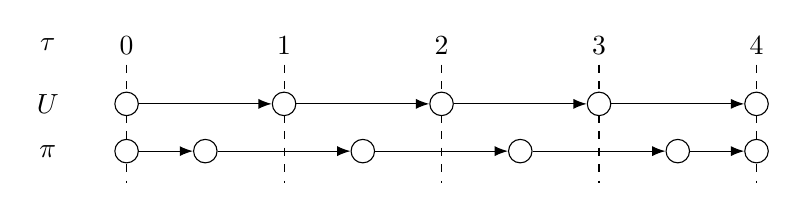
\begin{tikzpicture}[
        my-circle/.style={
            draw,
            circle,
            fill=white,
            inner sep=3pt,
        },
    ]
    \foreach \x in {0,1,...,4}
    {
        \draw[dashed] ($\x*(2, 0)+(0, 0.5)$) node[above] {$\x$} -- ++(0, -1.5);
    }

    \foreach \x in {0,2,...,8}
    {
        \node[my-circle] (link-\x) at (\x, 0) {};
    }

    \foreach \x in {1,3,...,8}
    {
        \node[my-circle] (momentum-\x) at (\x, -0.6) {};
    }

    \node[my-circle] (momentum-0) at (0, -0.6) {};
    \node[my-circle] (momentum-8) at (8, -0.6) {};

    \draw[->, >=Latex] (link-0) to (link-2);
    \draw[->, >=Latex] (link-2) to (link-4);
    \draw[->, >=Latex] (link-4) to (link-6);
    \draw[->, >=Latex] (link-6) to (link-8);

    \draw[->, >=Latex] (momentum-0) to (momentum-1);
    \draw[->, >=Latex] (momentum-1) to (momentum-3);
    \draw[->, >=Latex] (momentum-3) to (momentum-5);
    \draw[->, >=Latex] (momentum-5) to (momentum-7);
    \draw[->, >=Latex] (momentum-7) to (momentum-8);

    \node at (-1, 0.75) {$\tau$};
    \node at (-1, 0) {$U$};
    \node at (-1, -0.6) {$\pi$};
\end{tikzpicture}

\end{document}
